\section{Introduction}
\begin{frame}{Computational Solid Mechanics}
  \begin{minipage}{0.5\textwidth}
    \only<1>{
    \begin{block}{\color{White} Solid Mechanics}
      \begin{itemize}
        \item \color{Black} Relate deformation with internal force development
        \item $\boldsymbol{\nabla} \cdot \mathbf{P}= 0$ with \color{White} $\mathbf{P}=\mathcal{C}(\mathbf{F})$
      \end{itemize}
    \end{block}
    }
    \only<2>{
    \centering
    \includegraphics[width=0.85\textwidth]{Figures/intro/link}
    }
  \end{minipage}%
  \begin{minipage}{0.5\textwidth}
    \only<1>{
    \centering
    \includegraphics[width=0.85\textwidth]{Figures/intro/link}
    }
    \only<2>{
    \begin{block}{\color{White}Finite Element Method}
      \begin{itemize}
        \item General PDE solving method
        \item Discretize the domain 
        \item Weakly satisfy the PDE at selected points
      \end{itemize}
    \end{block}
  }
  \end{minipage}
\end{frame}

\begin{frame}{Composite Modeling}
  \begin{minipage}{0.5\textwidth}
  \only<1>{
    \centering
    \includegraphics[width=2\textwidth]{Figures/intro/scales}
    }
    \only<2>{
    \begin{block}{\color{White}FE$^2$}
      \begin{itemize}
        \item Representative Volume Element (RVE)
        \item Solve for RVE and average the response
        \item Repeat for every selected point
      \end{itemize}
    \end{block}
  }

  \only<3,4>{
  \begin{block}{\color{White}FE$^2$-Bottleneck}
      \begin{itemize}
        \item Micro-scale problem solution
        \item Repeating for every selected point
        \item Highly non-linear behaviour 
      \end{itemize}
    \end{block}
  }
  \end{minipage}%
  \begin{minipage}{0.5\textwidth}
  \only<2>{
    \centering
    \includegraphics[width=0.9\textwidth]{Figures/intro/FE2-CONV}
  }
  \only<3,4>{
    \centering
    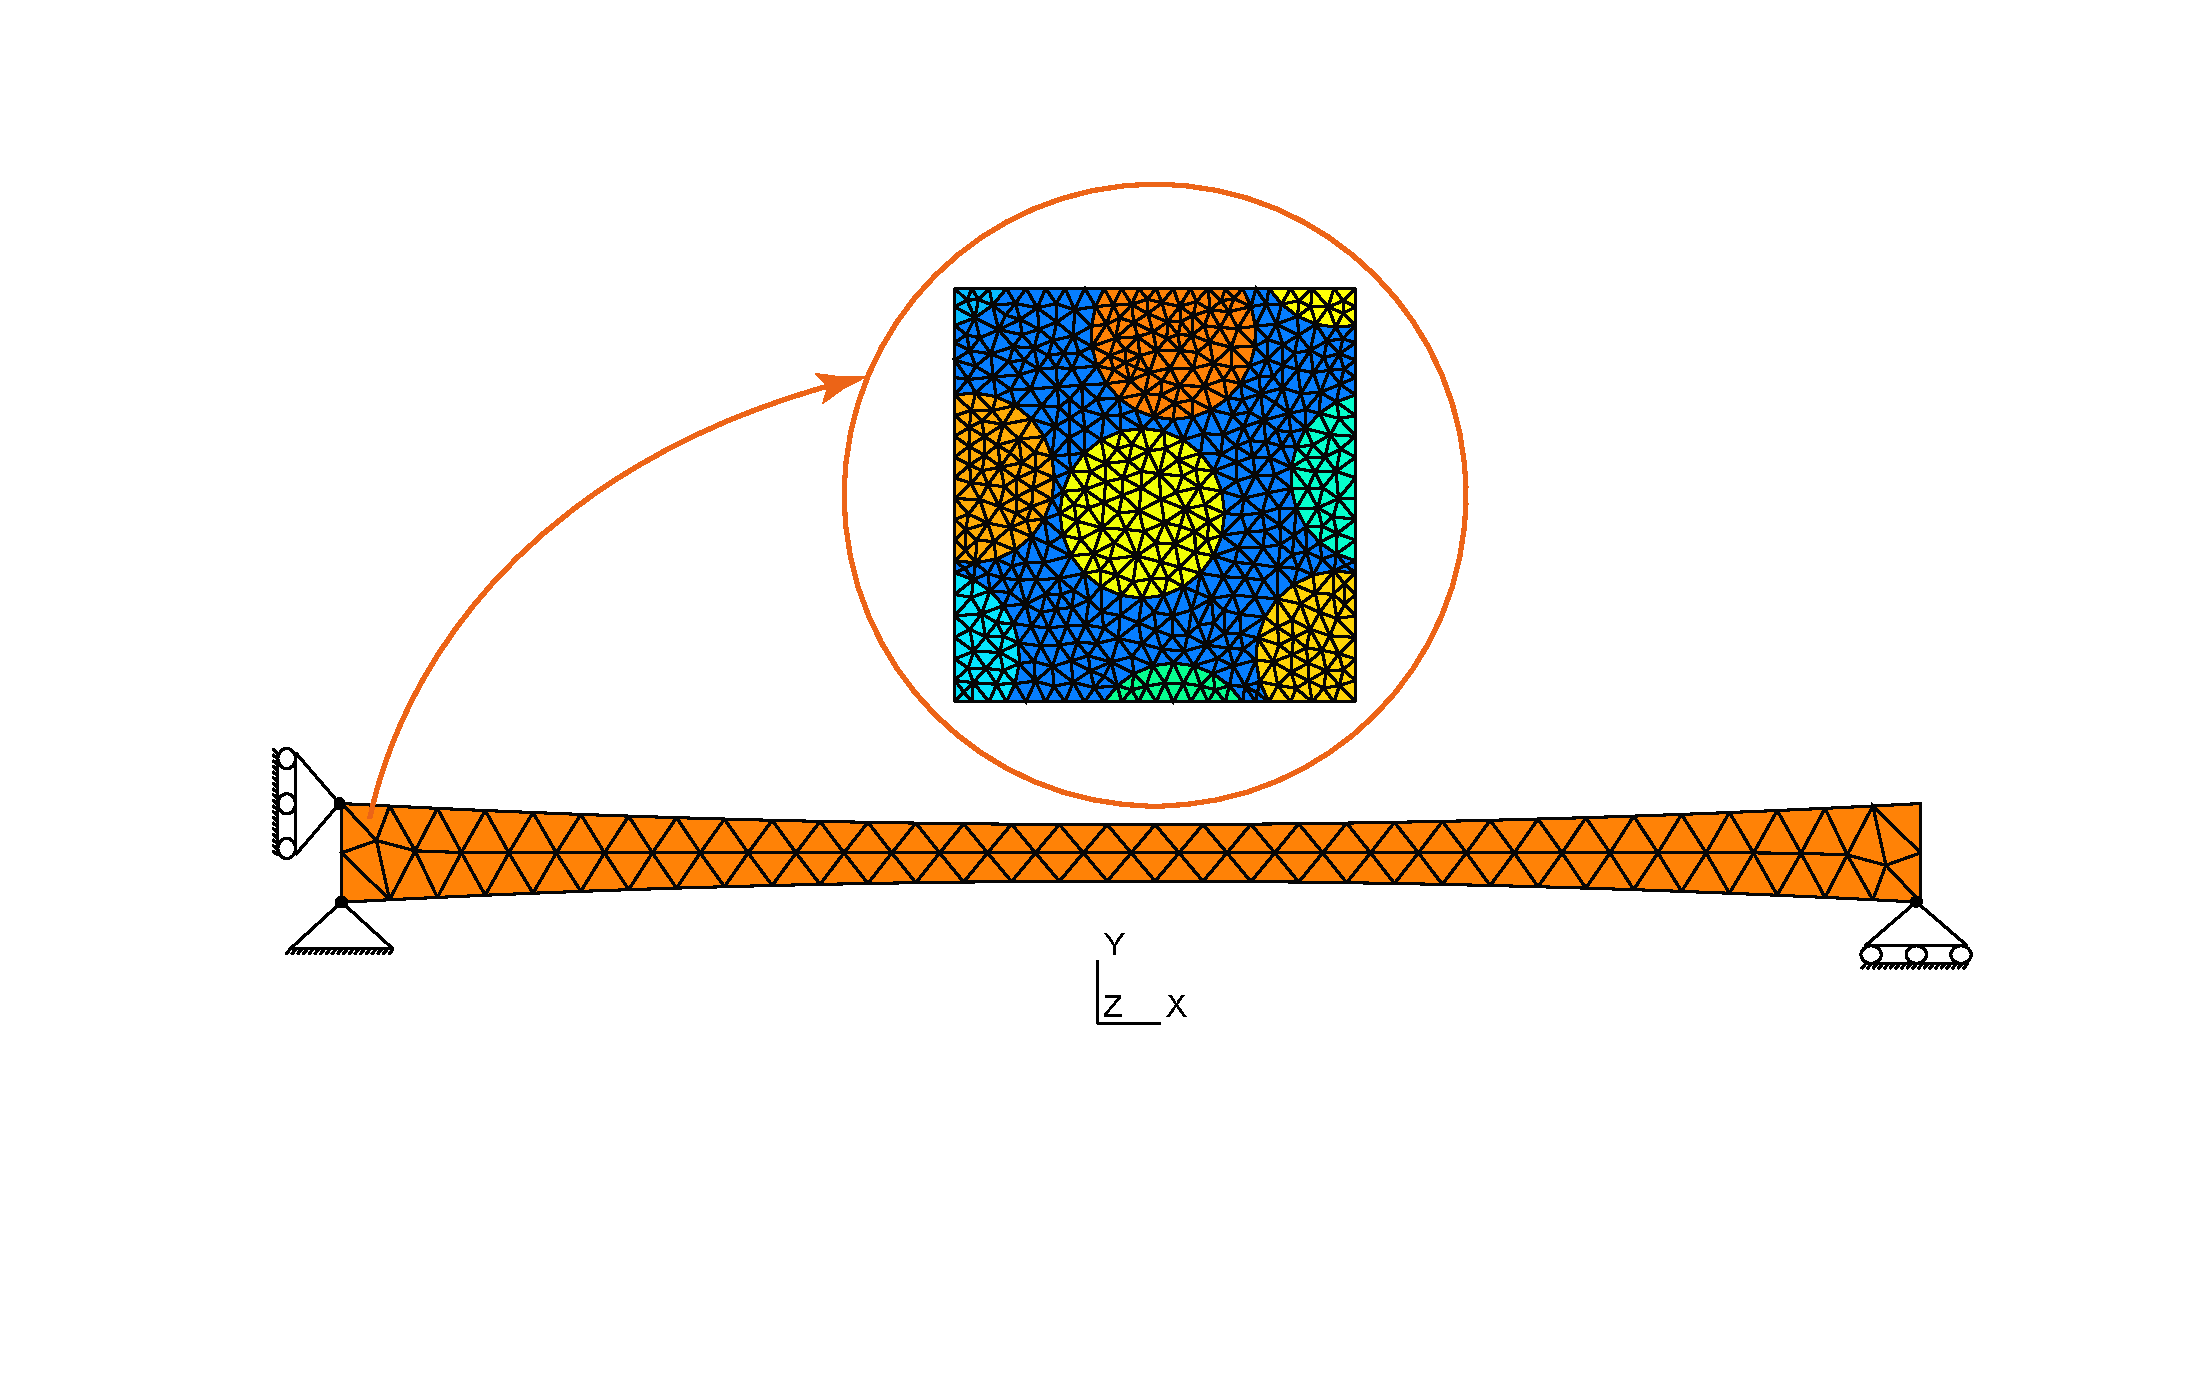
\includegraphics[width=\textwidth]{Figures/intro/bone}
  }
  \end{minipage}
  \only<4>{
    \centering
    \color{Pink} We need multiple of these simulations for real world applications!
  }
\end{frame}

